
% Cal Poly Thesis
% 
% based on UC Thesis format
%
% modified by Mark Barry 2/07.
%




\documentclass[12pt]{ucthesis}

%\newif\ifpdf
%\ifx\pdfoutput\undefined
%    \pdffalse % we are not running PDFLaTeX
%\else
%\pdfoutput=1 % we are running PDFLaTeX
%\pdftrue \fi

\usepackage{textcomp}
\usepackage{url}
\usepackage{listings}
\lstset{
    language=[Visual]C++,
    keywordstyle=\bfseries\ttfamily\color[rgb]{0,0,1},
    identifierstyle=\ttfamily,
    commentstyle=\color[rgb]{0.133,0.545,0.133},
    stringstyle=\ttfamily\color[rgb]{0.627,0.126,0.941},
    showstringspaces=false,
    basicstyle=\small,
    numberstyle=\footnotesize,
    numbers=left,
    stepnumber=1,
    numbersep=10pt,
    tabsize=2,
    breaklines=true,
    prebreak = \raisebox{0ex}[0ex][0ex]{\ensuremath{\hookleftarrow}},
    breakatwhitespace=false,
    aboveskip={1.5\baselineskip},
  columns=fixed,
  upquote=true,
  extendedchars=true
% frame=single,
% backgroundcolor=\color{lbcolor},
}
\usepackage{color}
%\usepackage{ifpdf}
%\ifpdf

    \usepackage[pdftex]{graphicx}
    % Update title and author below...
    \usepackage[pdftex,plainpages=false,breaklinks=true,colorlinks=true,urlcolor=blue,citecolor=blue,%
                                       linkcolor=blue,bookmarks=true,bookmarksopen=true,%
                                       bookmarksopenlevel=3,pdfstartview=FitV,
                                       pdfauthor=Ryan Schmitt,
                                       pdftitle=GPU-Accelerated Point-Based Color Bleeding,
                                       pdfkeywords={thesis, masters, cal poly, rendering, global illumination, GPU, acceleration}
                                       ]{hyperref}
    %Options with pdfstartview are FitV, FitB and FitH
    \pdfcompresslevel=1

%\else
%    \usepackage{graphicx}
%\fi

\usepackage{amssymb}
\usepackage{amsmath}
\usepackage[letterpaper]{geometry}
\usepackage[overload]{textcase}



\bibliographystyle{abbrv}

\setlength{\parindent}{0.25in} \setlength{\parskip}{6pt}

\geometry{verbose,nohead,tmargin=1.25in,bmargin=1in,lmargin=1.5in,rmargin=1.3in}

\setcounter{tocdepth}{2}


% Different font in captions (single-spaced, bold) ------------
\newcommand{\captionfonts}{\small\bf\ssp}

\makeatletter  % Allow the use of @ in command names
\long\def\@makecaption#1#2{%
  \vskip\abovecaptionskip
  \sbox\@tempboxa{{\captionfonts #1: #2}}%
  \ifdim \wd\@tempboxa >\hsize
    {\captionfonts #1: #2\par}
  \else
    \hbox to\hsize{\hfil\box\@tempboxa\hfil}%
  \fi
  \vskip\belowcaptionskip}
\makeatother   % Cancel the effect of \makeatletter
% ---------------------------------------

\begin{document}

% Declarations for Front Matter

% Update fields below!
\title{GPU-Accelerated Point-Based Color Bleeding}
\author{Ryan Schmitt}
\degreemonth{December} \degreeyear{2011} \degree{Master of Science}
\defensemonth{December} \defenseyear{2011}
\numberofmembers{3} \chair{Zo\"{e} Wood, Ph.D.} \othermemberA{Chris Lupo, Ph.D.} \othermemberB{Michael Haungs, Ph.D.} \field{Computer Science} \campus{San Luis Obispo}
\copyrightyears{seven}



\maketitle

\begin{frontmatter}

% Custom made for Cal Poly (by Mark Barry, modified by Andrew Tsui).
\copyrightpage

% Custom made for Cal Poly (by Andrew Tsui).
\committeemembershippage

\begin{abstract}

Traditional Global Illumination lighting techniques like Radiosity and Monte Carlo sampling are computationally expensive. This has prompted the development of the Point-Based Color Bleeding (PBCB) algorithm by Pixar in order to approximate complex indirect illumination while meeting the demands of movie production; namely, reduced memory usage, surface shading independent run-time, and faster renders than the aforementioned lighting techniques.

The PBCB algorithm works by discretizing a scene’s directly illuminated geometry into a point cloud (surfel) representation. When computing the indirect illumination at a point, the surfels are rasterized onto cube faces surrounding that point, and the constituent pixels are combined into the final, approximate, indirect lighting value. This algorithm achieves better performance than Monte Carlo ray-tracing, but we attempt to enhance it further.

Thus, in this thesis we present a performance enhancement to the Point-Based Color Bleeding algorithm through hardware acceleration; our contribution incorporates GPU-accelerated rasterization into the cube face raster phase. The goal is to leverage the powerful rasterization capabilities of modern graphics processors in order to speed up the PBCB algorithm over standard software rasterization. Our algorithm reproduces the output of the traditional PBCB technique, but reduces its run-time. We also compare our algorithm against our more accurate Monte Carlo tracing method in order to compare correctness.

\end{abstract}

%\begin{acknowledgements}

%   Thank you...

%\end{acknowledgements}


% \tableofcontents


% \listoftables

% \listoffigures

\end{frontmatter}

\pagestyle{plain}

\renewcommand{\baselinestretch}{1.66}


% ------------- Main chapters here --------------------

%---- Introduction ----
\begingroup
\chapter{Introduction}

%-------------------------------------------------------------------------------
% SECTION: Computer Graphics
%-------------------------------------------------------------------------------
\section{Computer Graphics}
Computer graphics is, in general, anything produced by a computer that isn't plain text or sound. Although, perhaps a more fitting definition is using a computer to draw a picture; this is also called rendering. There are a vast array of different areas in which one may want the help of a computer to render an image, from the entertaining, like video games and animated films, to the scientific, like medical visualization and computer-aided design and drafting. Each of these disciplines can have varying requirements of computer graphics: some need real-time rendering in order to respond to user-input, and others may trade the real-time speed for precise simulation. The goal of computer graphics is to identify the requirements of the application and render the highest quality image given those restrictions.

%-------------------------------------------------------------------------------
% SECTION: Ray-Tracing and Global Illumination
%-------------------------------------------------------------------------------
\section{Ray-Tracing and Global Illumination}
\label{sec:ray_tracing_intro}
In particular, this thesis is concerned with ray-traced rendering using Global Illumination algorithms, which are most commonly utilized to produce high-quality photo-realistic images. A ray-tracing algorithm can be classified as a Global Illumination algorithm when it incorporates not only direct illumination from light sources, but indirect illumination, or light that is inter-reflected between scene geometry from the same light sources (Figure \ref{fig:compare_illumination}).

\begin{figure}[h!]
    \centering
    \subfloat[Direct Only]{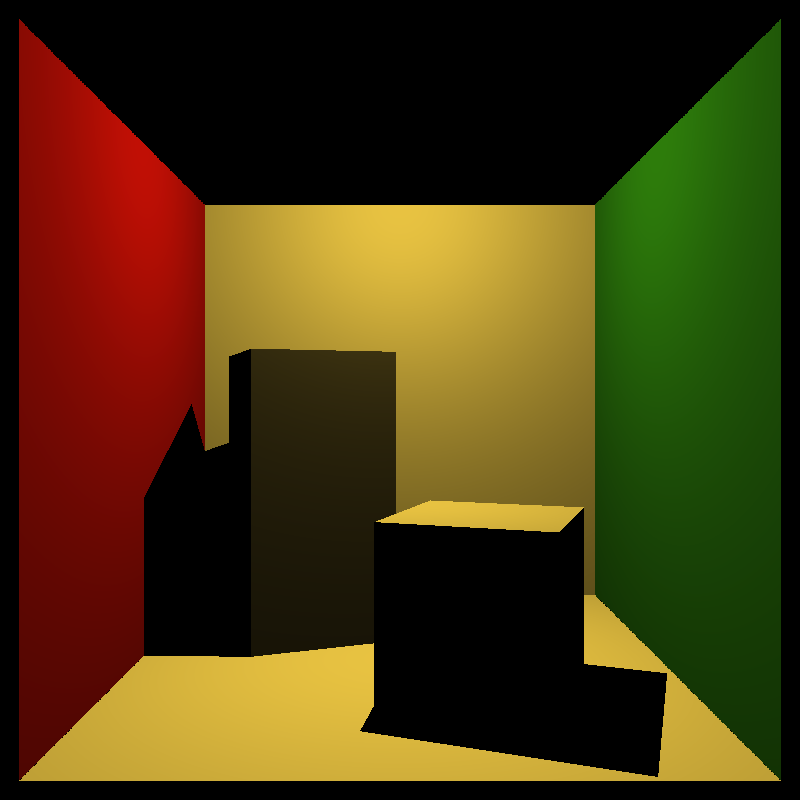
\includegraphics[width=70mm]{../img/cornell_simp_direct_only.png}}
    ~
    \subfloat[Direct \& Indirect]{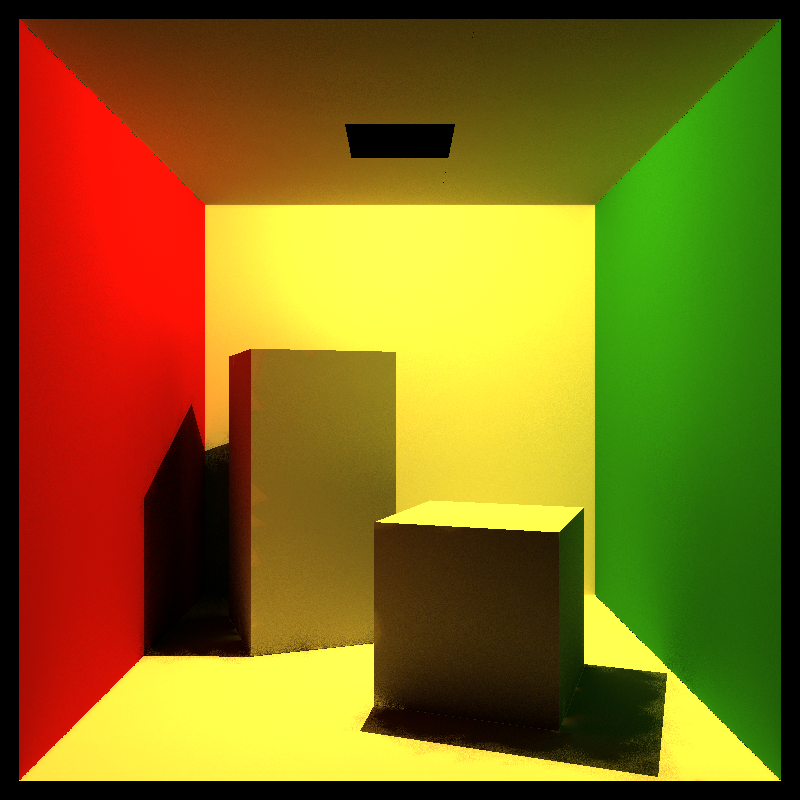
\includegraphics[width=70mm]{../img/cornell_simp_indirect.png}}
    \caption[Cornell Box direct \& indirect illumination]{Cornell Box rendered with both direct illumination and direct \& indirect illumination.}
    \label{fig:compare_illumination}
\end{figure}

Ray-tracing achieves photo-realism by simulating the physics of light using a scene comprised of light sources, mathematically-defined geometric surfaces, and a virtual camera (see figure \ref{fig:camera}). It produces renders that are specifically not real-time in nature, but meant to take as long as is necessary to produce quality results. In this setting, we must render life-like images, so an accurate simulation of light physics is required, but oftentimes we can obtain a convincing result using approximations. Specifically, ray-tracing follows the opposite path of the light: instead of tracing light rays from the light sources until they happen to hit the virtual camera, which is very physically accurate, we start at the camera and trace into the scene.

\begin{figure}[h!]
    \centering
    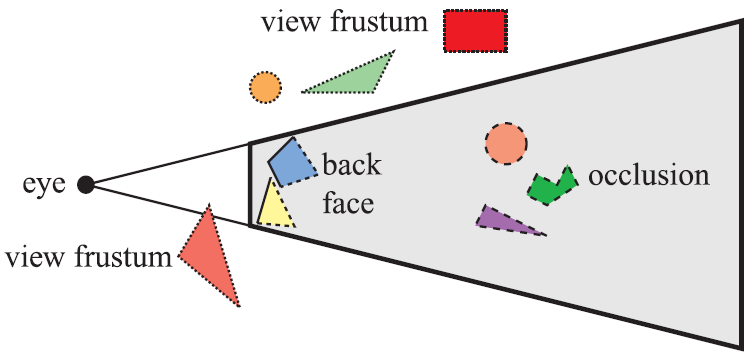
\includegraphics[width=100mm]{../img/RTR3_14_09_camera.png}
    \caption[Virtual camera, frustum, and geometry]{The eye and virtual camera are equivalent, geometry that lies in the viewing frustum is rendered. \cite{bib:rtr}}
    \label{fig:camera}
\end{figure}

Once these primary rays travel from the camera, into the scene, and intersect with the geometry, we can calculate the shading at that point in order to determine the color of the primary ray's associated pixel in the final rendered image. This shading calculation can vary from a simple direct illumination computation, to a complex Global Illumination calculation.

In this thesis, we focus on Global Illumination techniques. We split the calculation into direct illumination, which is the amount of light that leaves the source and directly intersects our shading point, and indirect illumination, which is the amount of light contributed from the diffuse inter-reflections of geometry in the scene; a phenomenon that is exemplified by the fact that the space under our desks is not completely dark, or that an illuminated red wall may reflect red light onto a nearby white box, causing it to appear reddish. These two components (direct and indirect illumination) are combined into one value that represents the incoming illumination at our primary ray's intersection point. We solve for the amount of this illumination that follows back along the ray to the camera, and we write that value to the primary ray's associated final-image-pixel. Performing this ray-tracing algorithm on each such final-image-pixel generates a rendering of the scene geometry as defined by the light sources and virtual camera, and is classified as Global Illumination.

%-------------------------------------------------------------------------------
% SECTION: Monte Carlo Ray-Tracing
%-------------------------------------------------------------------------------
\section{Monte Carlo Ray-Tracing}
\label{sec:monte_carlo}
One of the most widely used methods for the indirect illumination calculation in ray-tracing is called Monte Carlo sampling, and it involves randomly and discretely sampling the hemisphere above an intersection point (Figure \ref{fig:monte_carlo}). This is performed by recursively tracing yet more rays into the scene in order to gather information about what geometry is nearby and what color it is shaded; this attempts to solve for the diffuse inter-reflections incident at an intersection point. 

\begin{figure}[h]
   \centering
   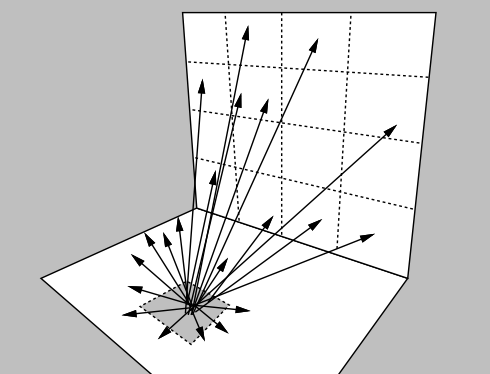
\includegraphics[width=80mm]{../img/shirley_monte_carlo.png}
   \captionfonts
   \caption[Monte Carlo hemisphere]{Monte Carlo sampling of a hemisphere above an intersection point \cite{bib:shirley1991}.}
   \label{fig:monte_carlo}
\end{figure}

Typically, around 128 of these rays are traced from each primary ray intersection point, into the scene, in order to gather enough shading information about the adjacent geometry to calculate a believable indirect illumination value. The number of rays that require intersection calculations, and shading calculations, can quickly escalate into the tens and hundreds of millions. Renders requiring multiple hours to complete are not rare.

%-------------------------------------------------------------------------------
% SECTION: Point-Based Color Bleeding
%-------------------------------------------------------------------------------
\section{Point-Based Color Bleeding}
Recently, the Point-Based Color Bleeding algorithm was developed at Pixar by Per H. Christensen \cite{bib:christensen2008} for indirect illumination. Instead of tracing rays, as in Monte Carlo ray-tracing, discretized surface elements (surfels) are rasterized onto a cube of eight-by-eight-pixel images, approximating the hemisphere used in the Monte Carlo ray-tracing (Figure \ref{fig:surfel_raster}). Once the surfels have been rasterized onto the pixels of the cube faces, the pixels are weighted and convolved into one value representing the indirect illumination at a point.

\begin{figure}[p]
   \centering
   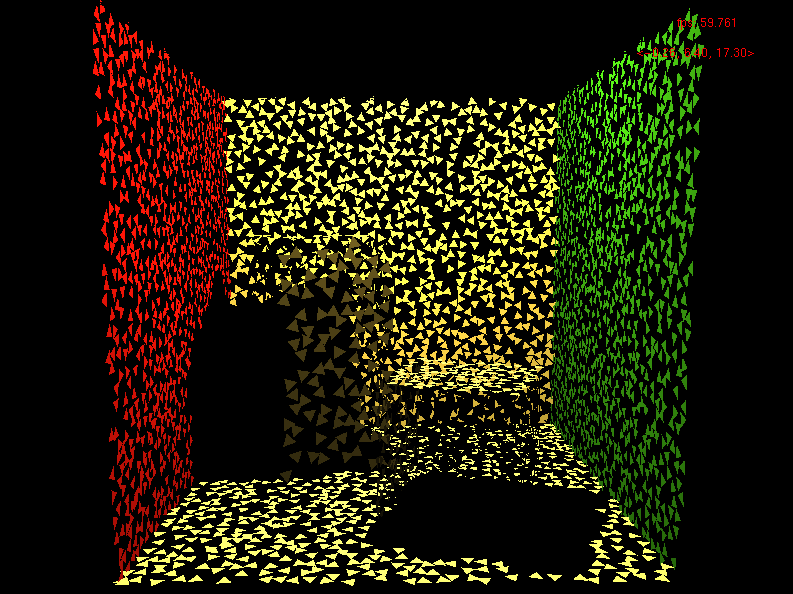
\includegraphics[width=130mm]{../img/surfel_cloud_tris.png}
   \captionfonts
   \caption[Cornell Box surfels]{Surfels for the Cornell Box scene. Note that the surfel size has been reduced to exhibit the sufel shape and distribution.}
   \label{fig:surfels}
\end{figure}

\begin{figure}[p]
   \centering
   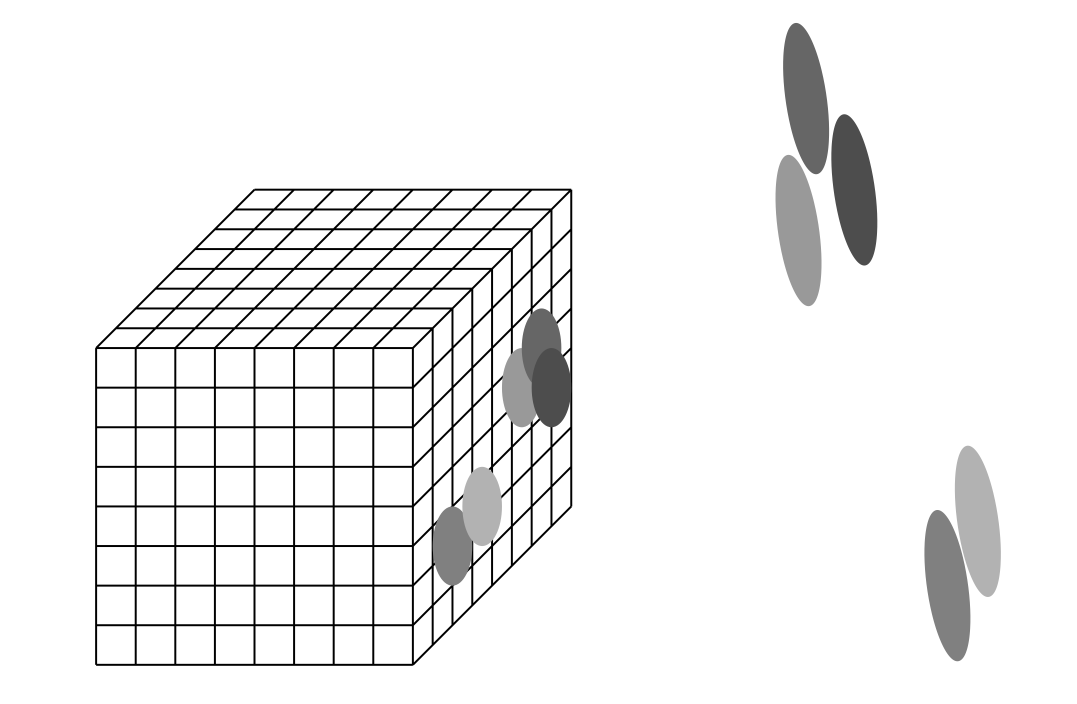
\includegraphics[width=100mm]{../img/surfel_raster.png}
   \captionfonts
   \caption[Rasterizing surfels]{Surfels being rasterized onto an 8x8 cube \cite{bib:christensen_slides}.}
   \label{fig:surfel_raster}
\end{figure}

The surfels are comprised of a location, surface normal, surface area, and shaded color computed from the direct illumination (Figure \ref{fig:surfels}). The benefit of this technique is that the surfels can be precomputed and stored in a point cloud, separate from the scene geometry, and reused. This lends itself well to reduced memory usage, surface shading independent run-time, and faster renders than Monte Carlo ray-tracing, all of which are very useful properties for Pixar and movie production in general.

%-------------------------------------------------------------------------------
% SECTION: Our Contribution
%-------------------------------------------------------------------------------
\section{Our Contribution}
This thesis is primarily concerned with performing the indirect illumination calculation faster than the Monte Carlo sampling method, without sacrificing render quality. We achieve this by extending PBCB to utilize the specialized rasterization capabilities of the modern heterogenous architecture chips' graphics processing unit (GPU) to rasterize the point cloud onto five eight-by-eight-pixel images arranged into a cube above each primary ray intersection point; this technique approximates the hemisphere that is used in the radiance integral (see section \ref{sec:radiance}). Also, we contribute a preprocess where the scene's geometry is transformed into triangles (the preferred geometric shape for GPU-rasterization) and assigned color values based on direct illumination calculations evaluated per triangle vertex.

\noindent In this paper, we:
\begin{itemize}
\item review important rendering related equations and techniques,
\item provide an in-depth description of the PBCB alrogithm,
\item present our PBCB extension and surfel generation preprocess,
\item discuss and analyze our validation techniques and results.
\end{itemize}

Our contributions, leveraging the modern heterogenous chips, realize much faster render times compared to Monte Carlo ray-tracing, while maintaining visually similar results (Figure \ref{fig:compare_techniques}). We achieve this by avoiding the numerous and costly intersection and shading calculations inherent in Monte Carlo Ray-tracing, and in some cases achieve an order of magnitude speedup.

\begin{figure}[h!]
    \centering
    \subfloat[Monte Carlo]{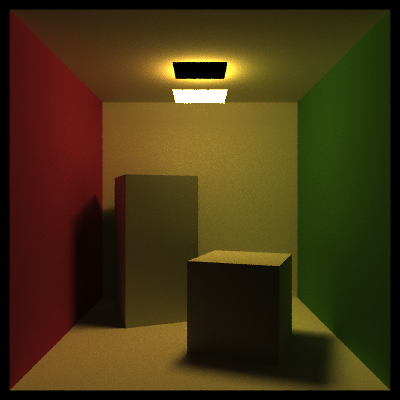
\includegraphics[width=70mm]{../img/cornell_simp_area_mcs.png}}
    ~
    \subfloat[GPU PBCB]{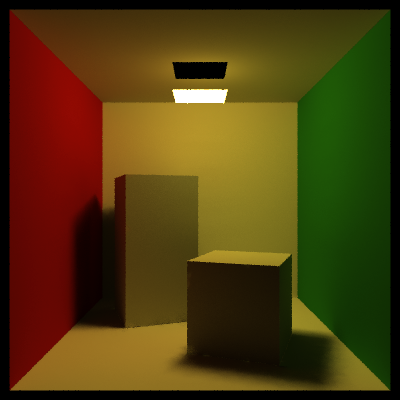
\includegraphics[width=70mm]{../img/cornell_simp_area_srf.png}}
    \caption[Cornell Box comparison]{Cornell Box with Indirect Illumination using both Monte Carlo Sampling and GPU PBCB.}
    \label{fig:compare_techniques}
\end{figure}


\endgroup

%---- Background ----
\begingroup
\chapter{Background}

%-------------------------------------------------------------------------------
% SECTION: Radiance
%-------------------------------------------------------------------------------
\section{Radiance}
\label{sec:radiance}

Radiance is a general term for the amount of light energy being transmitted through an area on a surface in a specific direction. Or more simply as the measure of brightness and color of a single ray of light \cite{bib:rtr}.

In order to understand how to calculate radiance, we must first understand radiant flux and flux density. Radiant flux, $\phi$, is a measure of energy (measured in joules) per second. Flux density is the instantaneous amount of radiant flux over an area, and is written as:
\begin{equation}
E = \frac{d\phi}{dA}
\label{eqn:flux_density}
\end{equation}
We can now define radiance as the flux density with respect to a projected area and a solid angle, or:
\begin{equation}
L = \frac{d^{2}\phi}{dA*\cos\theta*dw}
\label{eqn:radiance}
\end{equation}
Incoming radiance, or irradiance, is the radiance arriving at a surface, or the flux density of arriving light. We can define this in terms of radiance, where $x$ is a surface point and $w$ is the incoming ray direction, as:
\begin{equation}
E(x,w) = L(x,w) * \cos\theta * dw
\label{eqn:irradiance}
\end{equation}
Further more, we integrate over a hemisphere to solve for the incoming radiance, at point $x$, in all directions:
\begin{equation}
E(x) = \int L(x,w) * \cos\theta * dw
\label{eqn:irradiance_integral}
\end{equation}
Ultimately we are interested in the reflected radiance: the amount of irradiance that is reflected by a surface back towards our virtual camera. This is based on the material properties of the surface, which is typically represented by a BRDF (bi-direction reflectance distribution function). BRDFs are defined per-surface, and represented as $f(x, w^{\prime}, w)$. They solve for the ratio of radiance that is transmitted from an incoming direction, $w^{\prime}$, to an outgoing direction, $w$, at a surface point, $x$ (see figure \ref{fig:incoming_radiance}). Incorporating the BRDF, the equation for reflected radiance is:
\begin{equation}
L(p) = \int f(x, w^{\prime}, w) * L(p,w) * \cos\theta * dw
\label{eqn:radiance_integral}
\end{equation}

\begin{figure}
   \centering
   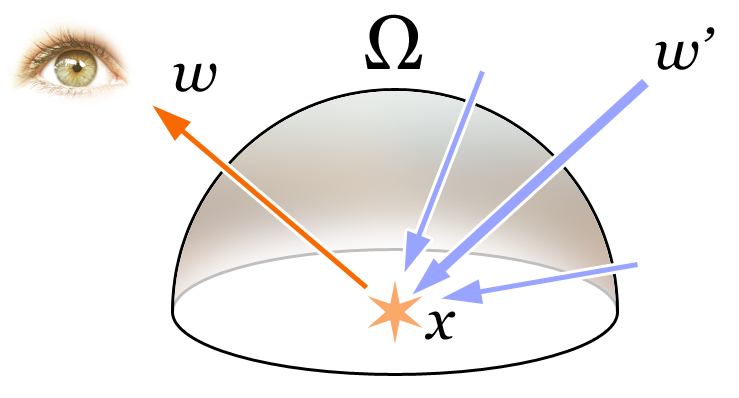
\includegraphics[width=100mm]{../img/rendering-equation-image.png}
   \captionfonts
   \caption[Incoming radiance hemisphere]{Incoming radiance in a hemisphere about a point, reflecting towards the camera. \cite{bib:nikishin_radiance}}
   \label{fig:incoming_radiance}
\end{figure}

%-------------------------------------------------------------------------------
% SECTION: Phong Reflection Model
%-------------------------------------------------------------------------------
\section{Phong Reflection Model}
\label{sec:phong_model}

The Phong reflection model is a simplified shading model used to calculate reflected radiance from one light source. It is most commonly used in scenarios that require fast computation, such as real-time graphics applications. It was presented by Phong in his University of Utah Ph.D. dissertation in 1973 \cite{bib:phong_thesis}. The equation calculates the reflected radiance using three color-vector terms: an ambient, diffuse, and specular.

The ambient component represents indirect illumination as a constant amount of reflected radiance added to all shaded points. This is the simplest term, but also poorly represents the subtleties of indirect illumination.

The diffuse component represents direct illumination using Lambertian reflectance of the incoming radiance. Lambertian refers to Lambert's cosine law, which states that, for perfectly diffuse surfaces, the diffuse reflected radiance is proportional to the cosine of the angle between the surface normal and the view vector, $\theta_{i}$. Figure \ref{fig:phong} visualizes these components.

\begin{figure}
   \centering
   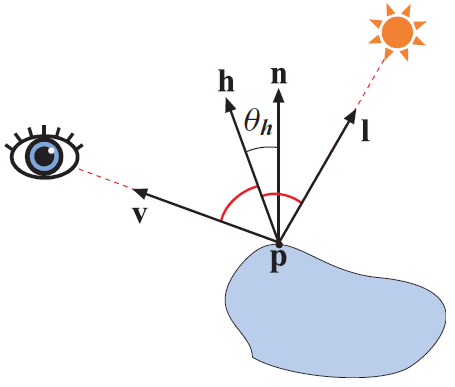
\includegraphics[width=100mm]{../img/RTR3_05_13_phong.png}
   \captionfonts
   \caption[Phong Shading Vectors]{The vectors involved in the Phong Reflectance Model. \cite{bib:rtr}}
   \label{fig:phong}
\end{figure}

The specular component represents the shininess we can view from certain angles on highly reflective surfaces. Specular reflectance is calculated by raising the cosine of the angle between the surface normal and the half vector (the vector halfway between the view and light vector), $\theta_{h}$, to the shininess of the surface, $s$.

Each of these components represent the ratio of incoming radiance, $C_{light}$ to reflected radiance, $C_{out}$, but the reflected radiance is also scaled by the surface material’s color characteristics, $C_{mat}$, as well as ambient, diffuse, and specular characteristics (represented by the scalar ratios: $M_{amb}$, $M_{diff}$, and $M_{spec}$, respectively). Combining these components we get the final Phong reflection model equation:
\begin{equation}
C_{out} = (M_{amb} * C_{mat} * C_{light}) + ((n \cdot l) * M_{diff} * C_{mat} * C_{light}) + ((n \cdot h) ^s * M_{spec} * C_{mat} * C_{light})
\label{eqn:phong}
\end{equation}

%-------------------------------------------------------------------------------
% SECTION: Anti-aliasing
%-------------------------------------------------------------------------------
\section{Anti-aliasing}
Anti-aliasing combats aliasing, the artifacting caused by under-sampling. A typical example of this in signal processing, where an analogue signal is sampled as some rate to determine it’s amplitude at that point in time. If the sample rate is too low (i.e. under-sampling) then the signal will not be accurately captured because the signal’s characteristics between samples was lost. This can be seen in Figure \ref{fig:undersampling}.

\begin{figure}[h!]
   \centering
   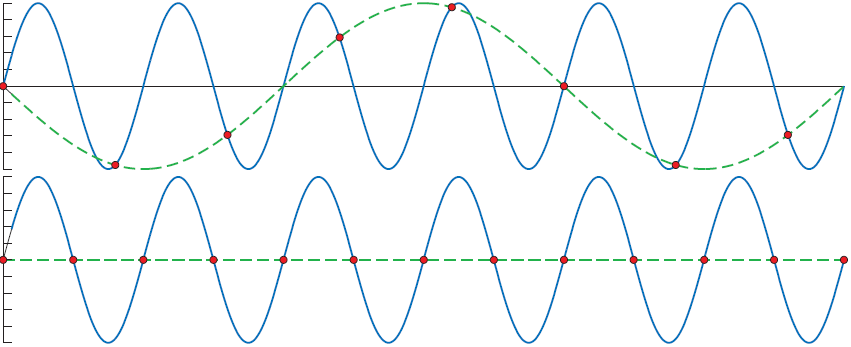
\includegraphics[width=100mm]{../img/RTR3_05_21_undersampling.png}
   \captionfonts
   \caption[Signal Undersampling]{The blue signals are being undersampled by the red dots, which leads to inaccurate reconstruction as evidenced by the dotted green line. \cite{bib:rtr}}
   \label{fig:undersampling}
\end{figure}

This occurs in computer graphics due to the limited sample rate provided by our display devices. To illustrate this point, imagine attempting to display a sphere with four pixels. More typically we experience aliasing in computer graphics as “jaggies,” or lines that should be smooth but are jagged (see Figure \ref{fig:jaggies}).

\begin{figure}[h!]
   \centering
   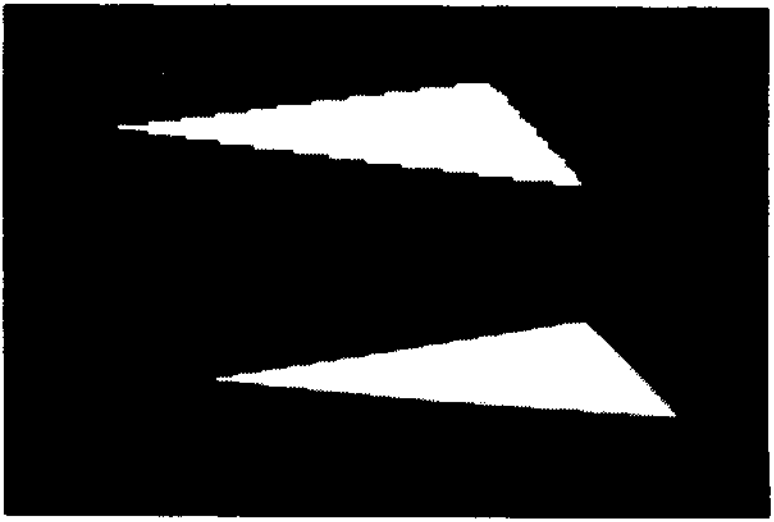
\includegraphics[width=100mm]{../img/jaggies.png}
   \captionfonts
   \caption[Jaggies]{Jagged edges apparent along the silhouette edges of the top triangle are reduced via anti-aliasing techniques in the lower triangle \cite{bib:crow1977}.}
   \label{fig:jaggies}
\end{figure}

In order to combat this phenomenon, techniques for anti-aliasing have been developed. These can take many forms \cite{bib:jimenez2011}, but generally it involves some form of over-sampling (i.e. rendering the image at a multiple of the display resolution) to compensate for the fixed sample rate of our display devices. By over-sampling the rendering, we can capture the subtleties of the image in software, and can down-sample the image in a way that helps alleviate the fixed display sample rate.

The simplest form of this technique is called super-sampling: where we render an image at some multiple of the desired final resolution, and down-sample the large image back to the desired final resolution by averaging the extra pixels into one value. For example, if we wish to render a 300 by 300 pixel image, we might render an intermediate image at 600 by 600 and then each final pixel is represented by 4 intermediate pixels, which can be averaged into one final pixel value; this is called 4x super-sample anti-aliasing.

However, in order to reduce the aliasing artifacts to an acceptable level, we usually require a large super-sample rate. This can result in unacceptably long render times. The main reason we require high super-sample rates in ray-tracing is the regular pattern  created by generating rays that pass through the center of each pixel. Generally in ray-tracing, the more random you can make a sample pattern (while not missing important features), the less aliased your final image will be. Therefore, we randomly jitter the direction of each ray within the bounds of the pixel. This facilitates lower super-sample rates.

An example image of anti-aliasing in our rendering algorithm can be seen in Figure \ref{fig:anti-aliasing}.

\begin{figure}[h!]
    \centering
    \subfloat[No Anti-aliasing]{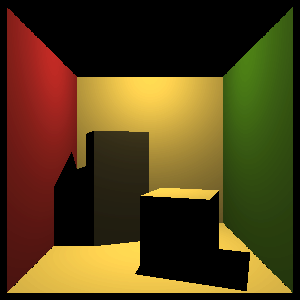
\includegraphics[width=70mm]{../img/cornell_simp_noAA.png}}
    ~
    \subfloat[9x Anti-aliasing]{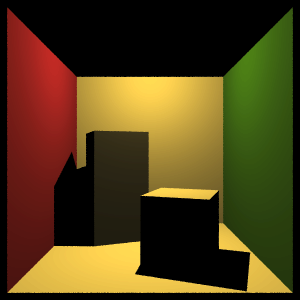
\includegraphics[width=70mm]{../img/cornell_simp_9xAA.png}}
    \caption[Anti-aliasing comparison]{Our simple Cornell box rendered with no anti-aliasing, and 9x box-filtered anti-aliasing.}
    \label{fig:anti-aliasing}
\end{figure}

%-------------------------------------------------------------------------------
% SECTION: Monte Carlo Integration
%-------------------------------------------------------------------------------
\section{Monte Carlo Integration}
\label{sec:monte_carlo_integration}

Monte Carlo integration is a technique used to evaluate integrals \cite{bib:pbr}. By repeatedly evaluating randomized discrete samples, we converge on the true evaluation of the integral. On average, these evaluations correspond to the correct solution, therefore we average multiple runs of the algorithm. We do not arrive at the correct solution in this way, but one that is statistically close.

We use Monte Carlo to evaluate the complex integral in Equation \ref{eqn:radiance_integral}. It is almost impossible to create a closed-form representation of the terms in this equation, and therefore Monte Carlo lends itself to its evaluation. To evaluate the incoming radiance at a point, we can generate randomized sample vectors (rays) over the domain of integration, the unit hemisphere. We then average these samples in order to obtain a result that is close to the true evaluation.

The main drawback of Monte Carlo integration is that it only converges at a rate of $O(n^{-1/2})$, with n being the number of discrete random samples. This means that increasing the number of samples by 4 would only reduce the error by half \cite{bib:pbr}. And because each sample requires one or more rays to be traced against the scene geometry and shaded at their intersection point, it quickly becomes cost-prohibitive to obtain low-error results. Error in this technique is exhibited by adjacent pixels that have disparity in their brightness and color, or noise.

Most of the current research in Monte Carlo for computer graphics is aimed at reducing this error through methods other than increasing the sample count \cite{bib:pbr}. One technique we use to better distribute the sample rays across the unit hemisphere is to discretize the hemisphere into a grid of sample directions with higher density in areas of higher importance, namely the top of the hemisphere where the $n \cdot l$ factor is largest, and jitter each sample direction by a random amount.

%-------------------------------------------------------------------------------
% SECTION: CPU versus GPU
%-------------------------------------------------------------------------------
\section{CPU versus GPU}
\label{sec:cpu_v_gpu}

due to their purpose. The CPU is considered a serial processor that handles general computation, which is typically thought of as instruction-driven, and involves executing unpredictable instructions on irregular data and likely includes branching. The GPU, on the other hand, is a stream processor optimized for data-driven graphics rendering of more regular data with predictable memory access. \cite{bib:rtr}

Because of their differing purposes, the CPU and GPU have traditionally been divided into two physically separate components of a computer system’s architecture connected by the PCI bus. The application running on the CPU will transmit rendering data and instructions over this bus to the GPU, which will process this input and produce a rendering. Depending on the purpose of this rendering, it can either be displayed on a monitor attached directly to the GPU, or transmitted back over the bus to the CPU for additional processing. As is common in multiprocessing systems, the two common problems we experience are load balancing and communication \cite{bib:rtr}. 

Load balancing can take place between the CPU and GPU, as well as internally within the GPU. The programmer is generally responsible for handing the load balancing between these two components, while the GPU itself leverages FIFO queues between stages to avoid stalling any part of the pipeline.

The latency and bandwidth of the bus connecting the CPU and GPU can cause communication problems as well. The theoretical maximum one-way bandwidth of the PCI Express 2.0 bus is 8.0 GB/s \cite{bib:pci_press}, while if we wanted to render 300 million triangles per second we would require a rate of 10.2 GB/s just to transfer the triangles to the GPU \cite{bib:rtr}. If we want to saturate this bandwidth, we must be constantly streaming data across the bus, however this is not always the use-scenario. Many times we wish to transmit data to the GPU, process it, and send it back to the CPU. In this case, the PCI bus can become the bottleneck as it is designed for one-way streaming of data.

%-------------------------------------------------------------------------------
% SECTION: Heterogenous Chip Architectures
%-------------------------------------------------------------------------------
\section{Heterogenous Chip Architectures}
\label{sec:heterogenous_chips}

The traditional architecture for systems with both CPU and GPUs involves the PCI bus, which connects two these two disparate components. However, recent advancements have allowed chip densities so high that both CPU and GPU can fit onto one silicon chip. These architectures, that combine CPU and GPU, are called heterogenous chips.

Intel has released both Sandy Bridge and, more recently, Ivy Bridge architectures \cite{bib:intel_press} that adhere to this ethos, and AMD has released Fusion \cite{bib:amd_press}. By combining both the CPU and GPU onto one chip, the hardware can bypass the shortcomings of the PCI bus to more quickly communicate.

In systems utilizing the traditional architecture, rendering small scenes that require final data processing on the CPU would have been cost-prohibitive due to the latency required to transfer data from CPU to GPU and back again. However, with heterogenous chip architectures, we can almost ignore this latency in our algorithms; allowing for new-found simplicity.


\endgroup

%% ------------- End main chapters ----------------------

\clearpage
\bibliography{thesis}
%\bibliographystyle{plain}
%%\addcontentsline{toc}{chapter}{Bibliography}

%\chapter{Related Work}
%
%\section{Global Illumination}
%Global illumination is an important field of study in computer graphics that numerous successful algorithms including photon mapping \cite{Jensen:2009}, radiosity \cite{radiosity} and Monte Carlo sampling techniques \cite{monte_carlo} try to mitigate or overcome in a reasonable time-frame.  Most commonly implemented methods are those that sample the scene and use a two phase approach (sample and gather) to model direct illumination and indirect illumination.  The gather stage included in most algorithms is built to be more efficient or lower resolution than the scene being rendered, which helps reduce the lighting computation cost.
%
%\subsection{PCB}
%Of particular relevance to this field is the work done in Point-Based Approximate Color Bleeding developed by Per Christensen \cite{christensen:2008}.  With this method, a subset of the scene geometry is thoroughly sampled, creating a point cloud representation of the direct lighting at each sample, which is then used to evaluate the incoming radiance surrounding a given point on a surface.
%
%As recently as 2010, discussion of approximating volume scattering using point clouds has been discussed \cite{christensen:siggraph}, however no specifics have been offered to how \textit{back-to-front or front-to-back rasterization} would be achieved with the current rasterization method (handled by our octree traversal method) or how scatter, extinction and absorption would be managed within the three-dimensional volume representation inside the point cloud.
%
%\subsection{Photon Mapping}
%Another closely related area of study includes photon mapping, a method that attempts to simulate light scatter and absorption properties of participating media, which has shown promise in the past.  In \cite{jensen:1998}, Jensen describes a process where photons participate and become stored inside the volume itself for later gathers during volume integration.  These photons are able to simulate scatter, absorption and passing through material (both geometric and volumetric.)
%
%While this technique is shown to work, it primarily focuses on caustic effects in volumes and the generated photon map.  Our storage method does not require data to be stored in the volume itself (as would be the case in photon mapping,) but in a separate, more lightweight data-structure better suited for out-of-core rendering.
%
%\begin{figure}[h!]
%    \centering
%    \includegraphics[width=100mm]{img/external/ewr7_mcbox.jpg}
%    \caption{Global illumination example achieved via photon mapping.  Source: http://graphics.ucsd.edu/\string~henrik/papers/photon\_map/}
%    \label{fig:photon}
%\end{figure}
%
%\section{Volume Rendering}
%This paper is focused on the lighting and rendering of scenes which contain volume data.  A number of approaches have been developed in order to represent volume data through computer visualizations or renders~\cite{Kajiya84},\cite{levoy88}.
%
%\subsection{Existing Work}
%Some of the first proposed volume rendering and shading techniques are described in \cite{levoy88}.  Before the time of the paper's creation, many of the accepted methods of volume visualization involved generating polygonal representations of the volumes by sampling the opacities and comparing them to a selected isovalue to determine whether or not the voxel is designated as ``inside'' the volume or ``outside.''  A polygonal mesh is then constructed based on this differentiating boundary.  Unfortunately, the algorithm defined above fell prey to spurious surfaces and holes caused by a limited sample range (since the polygonal method suffered from having to make a binary decision.  Either a ray intersected the volume or it did not.)
%
%In response to this, Levoy proposed a process of testing against two arrays (one with opacities and one with colors) that represent the voxel data-structure.  If a voxel was intersected, the algorithm would interpolate its color and opacity to those surrounding it based on the nature of the intersection.  This allowed for transparent volumes, and also allowed for opacities to be separated from voxel color, allowing for some important pre-processing to be done on the data such as volume classification, where the opacity of a volume is determined on an iso-range.  This in turn allowed the renderer to focus attention to specific densities in scans (useful for medical imaging.)
%
%\begin{figure}[h!]
%    \centering
%    \includegraphics[width=100mm]{img/external/img188.png}
%    \caption{Volume renders from \cite{levoy88} showing CT scan volume data visualized in three-dimensions, complete with realistic lighting. }
%    \label{fig:levoy}
%\end{figure}
%
%\subsection{Multi-Resolution Volumes}
%Because of the complexity of volume data (both through data representation and computation,) volume rendering algorithms often implement efficient multi-resolution data representation~\cite{Westermann94}.  \cite{Levoy90} describes a hierarchical method of managing a volume data set in order to remove unnecessary ``Empty'' cells and to reduce the amount of intersection tests done on voxels (or ``Cells'', as the higher level nodes are referred to.)  This algorithm introduced the use of octrees as an efficient means of dividing and containing the volume data.
%
%Our algorithm implements a sparse octree data-structure for both the volumes in the scene and the point-cloud used for the indirect lighting equation.
%
%\subsection{Occlusion Techniques}
%Another method to accelerate volume rendering involves estimating what nodes in a volume octree are definitely occluded based on surrounding node densities.  \cite{guthe} describes building a two-dimensional occlusion map and filling it in over a series of iterations, removing occluded nodes from being tested each iteration.  This method has been shown to drastically increase rendering performance by removing as much as 30\% per iteration.
%
%Based on many existing volume rendering algorithms, our implementation takes advantage of a multi-resolution, view-independent octree data-structure in order to handle a large amount of complex lighting and volume data.  We then use this very same octree representation to evaluate occluded regions, skipping scene data occluded by opaque geometry cached in the data-structure in the form of surfels.
%
%\subsection{Volume Lighting}
%As our computational power has improved, we have been able to tackle problems in lighting that we could not have overcome in the past.  \cite{kniss:03} builds upon Levoy's volume rendering method by implementing shadowing by sending shadow rays toward each light for each sample within the volume in order to estimate the amount of extinction between the point and the light.  Indirect lighting is also employed (though only forward-scattering due to the incremental nature of their algorithm.)
%
%\cite{zhang} attempts to handle multiple-scattering and volume shadows in scenes that sport mixed polygonal and volumetric data.  The paper describes light scatter representations similar to Equations \ref{siga_eq}, \ref{sigs_eq}, \ref{eq:sigt}, where light is able to scatter in and out from the sampling ray.  The algorithm then handles volume shadows caused by polygonal mesh data by constructing a series of shadow buffers, evaluating the volume shadow as a texture at each slice.
%
%While our volume lighting equation takes into account volume scatter properties, we do not evaluate shadows in a separate pass.  Instead, our algorithm not only evaluates transmittance between arbitrary sample points and the scene lights (giving us believable direct lighting), but we simulate scatter in properties by casting Monte Carlo samples out into our point-cloud to evaluate scene and volume radiance.  Additionally, our point cloud is not constrained by our traversal method, so all forms of scatter are supported.  Finally, the algorithm described also does not handle scatter out contributions to the scene, where the volume data may contribute to the rest of the scene's lighting.
%
%%==============================================================================%
%\chapter{PCB Extension Algorithm}
%\label{algorithm_sec}
%We present an algorithm which is an extension to the point cloud techniques described in \cite{tabellion} and \cite{christensen:2008}, specifically building off the point-based color bleeding (PCB) technique by Christensen.  The modifications involve evaluating light scatter and absorption properties at discrete points in the volume and adding them to the point cloud.  Using a front-to-back traversal method, we can correctly and quickly approximate the \textit{light-volume} representation's contribution to a scene's indirect lighting evaluation.
%
%\section{Point Based Color Bleeding}
%
%\begin{figure}[h!]
%    \centering
%    \includegraphics[width=100mm]{img/pcloud.png}
%    \caption{An example of a point-cloud scene where the geometry had been sampled, a disc representation replacing the geometry.  The radii of the discs in this image are reduced to better exemplify their presence.}
%    \label{fig:pcloud}
%\end{figure}
%
%In general, the color-bleeding algorithm subdivide the world into small representational segments, called surfels in \cite{christensen:2008}, which are stored in a large point cloud, representing the scene (See Figure \ref{fig:pcloud}.)  Surfels are used to model direct illumination, and are then used in a later phase to compute indirect lighting and color bleeding in an efficient manner.  This method is split up into three stages:
%
%\begin{enumerate}
%\item Sample the scene and save a discrete representation of the surfaces along with direct lighting in a point cloud
%\item Perform normal ray tracing on the scene geometry
%\item Replace ambient estimates with a gather stage, sampling the scene around a point to gather the indirect lighting component
%\end{enumerate}
%
%The goal of our proposed method is to include volumetric representations into a global illumination algorithm in a fast and coherent way similar to how surfels are represented in the point cloud.
%
%\section{Extension Overview}
%
%In the existing algorithms~\cite{christensen:2008}, surfels represent opaque materials within the point cloud.  Thus to incorporate a representation of volumetric data, an additional data representation was necessary to handle the scatter and absorption properties of participating media.  In general, our data representation closely follows the model of surfels, in that we choose to sample the volume at discrete locations and store a finite representation of the lighting at those discrete locations, but with modifications to handle the special attributes of lighting in transparent media.  In keeping with the naming conventions established, we call our discrete sampling of lighting elements for a volume: \emph{lvoxels}.  
%
%As a quick review, our algorithm must do the following:
%\begin{enumerate}
%\item Sample the scene geometry and store the direct lighting (or relevant lighting properties) within an acceleration structure for fast evaluation
%\item Sample the participating media and evaluate scatter, absorption and direct lighting at each discrete point
%\item Identify points of interest during regular ray casts using scene geometry 
%\item Orient a set of hemispherical samples along the normals of ray cast surfaces and cast the rays into the point-cloud
%\item Model the scatter-out and scatter-in properties of volumetric lighting during the indirect lighting gather stage.
%\end{enumerate}
%
%\section{Sampling the Scene}
%The goal of this stage of the algorithm is to sample the scene geometry (including the volume) and store the direct lighting in a finite data representation to be used later for global illumination lighting effects.  As all of our finite data represents the direct lighting of some small portion of a surface or element in a three-dimensional scene, we refer to the union of all finite lighting samples as a ``point cloud''.  This point cloud is stored in an octree representation for efficient access to all data elements, surfels and lvoxels.  Surfels differ from lvoxels only in that surfels represent a flat, solid geometry while lvoxels represent a transparent, volumetric medium.  Both have radii and position so both can be placed within the same point cloud.  
%
%\begin{figure}[h!]
%    \centering
%    \includegraphics[width=100mm]{img/diag/surfel_samp.pdf}
%    \captionfonts
%    \caption{Rays are cast from a special camera during the surfel sample phase.  Each time the ray intersects with geometry a surfel is created.}
%    \label{fig:surf_sample}
%\end{figure}
%
%\subsection{Surfel Sampling}
%
%We sample the opaque geometry in surfels, which are computed using an abstract sampling camera with a field of view slightly larger then the current viewing frustum, with a sampling rate two times that of the desired pixel resolution.  Rays are cast from the sampling camera and intersections with geometry mark sample points as seen in Figure \ref{fig:surf_sample}, giving the scene a view-dependent, thorough sample set.
%
%\subsection{LVoxel Sampling}
%
%Lvoxels are generated by marching over the entire domain of the volume by a specific, preset interval, sampling scatter and absorption coefficients in order to get an average throughout the area an lvoxel will occupy.  Typically this involves eight to sixteen absorption and scatter samples per lvoxel.  These values, as well as the radius of the lvoxels, may differ depending on the complexity and raw resolution of the volume.
%
%Caching the direct light contribution at each lvoxel by testing the transmittance using Equation (\ref{transmittion_eq}) to each light source saves us from re-computing light calculations during sampling in sections \ref{scatterout_sec} and \ref{scatterin_sec} \cite{signotes:2010}.
%
%\section{Gathering Light}
%
%\begin{figure}[h!]
%    \centering
%    \includegraphics[width=80mm]{img/diag/orthnormal.pdf}
%    \captionfonts
%    \caption{Basis vectors are generated based on the surface normal in order to transform samples on a hemisphere to test surrounding radiance.}
%    \label{fig:orthonormal}
%\end{figure}
%
%\subsection{Point-Cloud Ray Casting}
%
%Next, our algorithm uses a gather stage similar to the one in PCB, which calculates the irradiance at a point on a surface, given the radiance of the scene around it.  Unlike PCB, which uses a software rasterization method, we chose to evaluate irradiance by ray casting into the point-cloud around a hemisphere oriented along the surface's normal.  The decision to cast out of a hemisphere rather than using a software rasterization technique as was adopted in previous PCB implementations was made to simplify the tests which compare traditional Monte Carlo sampling methods to the extended PCB algorithm, but also to simplify evaluation of the transparent lvoxels within the octree.
%
%\subsection{Hemisphere Sampling}
%
%In order to approximate the integral of incoming light at point $p$ on the surface, we sample across a hemisphere oriented along the surface's normal $N$ at $\textup{p}$ as seen in Figure \ref{fig:orthonormal}.  This process is broken down into two distinct steps:
%
%\begin{enumerate}
%    \item The rays must sample across a hemisphere in an equally distributed fashion in order to gain an acceptable sampling of the surrounding radiance
%    \item Each sample ray must then be transformed based on the intersection surface's normal
%\end{enumerate}
%
%It is necessary to consider the sampling method just as important as the evaluation of those samples.  Generating purely random rays leads to clumping and high levels of noise, so a stratified sampling method was chosen, subdividing the sample space equally into a two-dimensional grid and jittering within the grid.  This helps us avoid clumping issues, and guarantees an even distribution over the entire domain.  In order to map this two dimensional domain over our hemisphere, we chose the following mapping code (converted from a function over spherical coordinates):
%
%% (based off of a cosine weighted hemisphere sampling method in Physically Based Ray Tracing \cite{pbrt})
%
%\begin{lstlisting}
%Vec3 sampleToHCoord(float us, float ts) {
%    const float r = sqrt(1. - us);
%    const float theta = 2 * PI * ts;
%    const float x = r * cosf(theta);
%    const float y = r * sinf(theta);
%    return Vec3(x, y, sqrt(us));
%}
%\end{lstlisting}
%
%Note that $sqrt(us)$ represents the Z value of the hemispherical sample (with the normal naturally placed down the Z plane.)  $sqrt(1. - us)$ represents the radius and $ts$ covers the theta (or angle around the normal of the hemisphere.)
%
%In order to force a regular distribution over this mapping equation, we chose to employ a common sampling technique over $us$ and $ts$, whose domains both ranged from 0.0 to 1.0.  We implemented a form of stratified stochastic sampling, which involves subdividing the domains into smaller sub-domains and randomly sampling within each sub-domain.  The major benefit to stratified stochastic sampling is the promise that the random samples are separated in their own sub-domains and are thus less likely to clump, giving us a better overall sampling over each domain.
%
%\begin{figure}[h!]
%    \centering
%    \includegraphics[width=80mm]{img/diag/gather.pdf}
%    \captionfonts
%    \caption{Gather rays are cast into the point-cloud, returning the estimated radiance coming from a given direction.  The radiance is then scaled based on the solid angle of that sample cast (based on sample count.)}
%    \label{fig:gather}
%\end{figure}
%
%In Section \ref{sec:int_vol}, we will employ a similar technique for sampling over volumes, but instead of sampling over hemispheres, we will sample over the domain of a sphere.  Therefore, the only necessary change is to our mapping function.  We remap $us$ to span from a range from -1.0 to 1.0, taking into account both hemispheres of the sphere.  The rest of the mapping function is basically the same:
%
%\begin{lstlisting}
%inline Vec3 sampleToSCoord(float us, float ts) {
%    const float z = 1.f - 2.f * us;
%    const float r = sqrt(max(0.f, 1.f - z * z));
%    const float phi = 2.f * PI * ts;
%    const float x = r * cos(phi);
%    const float y = r * sin(phi);
%    return Vec3(x, y, z);
%}
%\end{lstlisting}
%
%Now that we have an equally distributed set of rays over the hemisphere, we must orient all of them by the normal of the intersected surface.  We do this by creating an orthonormal basis matrix using the normal as our projected Z axis.  This matrix is saved for later when we apply the matrix to the sample rays.
%
%\begin{lstlisting}
%void orient(Vec3 normal) {
%    Vec3 up = Vec3(0,1,0);
%    Vec3 w = normal;
%    Vec3 u;
%    Vec3 v;
%    w.norm();
%    if(w.y() >= 0.9995 || w.y() <= -0.995) {
%        u = Vec3(1,0,0);
%        v = Vec3(0,0,1);
%    }else{
%        up.cross(w, &u);
%        u.norm();
%        w.cross(u, &v);
%    }
%
%    MyMat m = MyMat(u.x(), v.x(), w.x(), 0,
%                    u.y(), v.y(), w.y(), 0,
%                    u.z(), v.z(), w.z(), 0,
%                    0,     0,     0,     1);
%}
%\end{lstlisting}
%
%Each sample cast out from $p$ evaluates $L(\textup{p} \leftarrow w)$ (as shown in Figure \ref{fig:gather},) which is then multiplied by the scalar $w \cdot N$ in order to represent $cos\theta$.  In order to obtain good results, 128-256 samples are typically necessary to combat noise caused by the samples.  The resulting irradiance from the weighted sum of the samples is normalized by multiplying the normalization factor for the given phase function.
%
%%The \textit{probability density function} (PDF) describes the relative probability of a random variable taking on a particular value, and is important 
%
%%Applying these samples is a trivial matter, as each sample contributes according to the area of the cone of which that sample represents.  It is important to remember that these samples are estimating an integral that evaluates to 1.  With this in mind, consider the following equation, where $\theta_{max}$ is considered the max divergence from our surface normal.
%
%
%%\begin{equation}
%%\mathit{p}(x) = \frac{1}{Area_{cone}} = \frac{1}{Area_{hemisphere} * Fraction_{cone}} = \frac{1}{2\pi(1 - \textup{cos}\theta_{max})}.
%%\label{eq:source}
%%\end{equation}
%
%%Which leaves us with a PDF of $\frac{1}{2\pi}$, a value 
%
%\section{Integrating Volume Data}
%\label{sec:int_vol}
%In order for \textit{lvoxels} to contribute meaningfully to our scene during the light gather stage, we must make some architectural modifications to the algorithm in order to handle 1) more than one sample type in our octree and 2) the ability to handle non-opaque samples.  Both of these required simple changes in the octree data-structure as well as modification of the traversal algorithm used.
%
%\subsection{Data-Structure Modifications}
%Modifications to the previously mentioned irradiance sampling technique in order to allow scatter-out effects with volumes are few.  The biggest changes are to the point cloud octree and its traversal.  Specifically, when computing lighting, we must account for the fact that when an element of the point cloud is hit, it may be transparent.  In the standard algorithm, absorption and transmittance would not be taken into account and the traversal would stop at the first lvoxel encountered.
%
%Therefore, our algorithm must fulfill the following requirements: 1) The algorithm must ensure that the \textit{lvoxels} are placed in the same octree data-structure as the \textit{surfels}, 2) Our algorithm must keep track of the current Transmittance in order to determine the contribution of all samples encountered and 3) We must traverse the leaf nodes of the scene from front-to-back in order to integrate transparent sample contributions correctly.
%
%\subsection{Octree Traversal}
%
%In order to properly evaluate transparent and opaque surfaces within the point cloud, we made changes to node-level octree traversal.  Each branch traverses its children from closest to farthest, guaranteeing that closer leaf nodes are evaluated first.  Leaf nodes then use the pre-evaluated scatter ($\sigma_{s}$) and absorption ($\sigma_{t}$) coefficients for each lvoxel to appropriately alter the sample ray's transmittance, and continue with the traversal, with each hit contributing to the final resulting radiance value.  Once a surfel is hit, there is no need to continue traversing the octree as seen in Figure \ref{fig:testing}.
%
%\begin{figure}[h!]
%    \centering
%    \includegraphics[width=100mm]{img/testing.png}
%    \caption{Illustrates the octree traversal algorithm testing efficiency.  Lighter shades represent less tests, while darker shades represents the most.  Closer objects evaluate faster, and all data in the point-cloud behind them are occluded.}
%    \label{fig:testing}
%\end{figure}
%
%%------------------------------------------------------------%
%\subsection{Acquiring Scatter-Out Contributions}
%\label{scatterout_sec}
%
%Once the changes to the point-cloud data-structure have been made, we are able to 1) ensure correct evaluation of the transparent surfaces through front-to-back octree traversal and 2) stop evaluating leaf nodes once we have hit an opaque surfel, reducing the overall sample count.  Now that \textit{lvoxels} are supported, we simply sample the scene as we have with regular PCB.  The modified traversal algorithm already takes care of transmittance through any transparent media so no further changes are necessary.
%
%%------------------------------------------------------------%
%\subsection{Acquiring Scatter-In Contributions}
%\label{scatterin_sec}
%After adding lvoxels to our octree structure and evaluation algorithm, the only modifications necessary for scatter-in are within the volume rendering equation.  As an overview, volume integration will step through the volume, at each point it will:
%
%\begin{enumerate}
%\item Update the current transmittance by the scatter and absorption terms at the given point
%\item Cast shadow rays to estimate the direct light (and in cases of non-uniform scatter, apply a phase function)
%\item Sample scatter contribution by sending rays out into the point cloud
%\item Add direct illumination contribution and indirect illumination to the current incoming radiance
%\end{enumerate}
%
%In order to model lighting for a volume, in-scattering requires integrating over all directions (over the domain of the surrounding sphere.)  Casting Monte Carlo sample rays through the volume and into the scene would be computationally expensive, specifically because we would be almost guaranteed to integrate over the volume at every sample.  Instead, for each sample we send out rays into the point cloud, iterating through a much less dense dataset like in Figure \ref{fig:scatter_in}.  This dataset represents the volume and the surrounding polygonal geometry, giving us the indirect lighting component from both simultaneously.
%
%This method helps us replace expensive $S(\textup{p, w})$ evaluations with traversals into the octree.  The two main differences between sampling scattered light within a volume and evaluating the irradiance on a surface are 1) the distribution function, which is based on the volume's phase function, and 2) the samples are distributed over a sphere rather than a hemisphere.
%
%These scatter samples are distributed throughout the volume marching process typically taken while rendering volumes as seen in Figure \ref{fig:vol_step}.  More specifically, a single spherical sampler is kept throughout the integration of the volume over the ray.  This sampler keeps track of eight sub-samplers, each given a portion of the overall spherical domain.  For each sample step, one of the eight subsamples is randomly chosen to generate sixteen rays to cast into the scene.  The overall effect is an eventual distribution of rays over the sphere across four to eight sample steps.  We found that the sample steps were small enough that the difference in location was minuscule.  These sample points then gather from the point cloud like traditional sample rays.
%
%
%\begin{figure}[h!]
%    \centering
%    \includegraphics[width=90mm]{img/diag/scatter_in.pdf}
%    \captionfonts
%    \caption{Sample rays are cast during volume traversal, allowing for decent estimates of lighting contribution at each point.}
%    \label{fig:scatter_in}
%\end{figure}
%
%
%\begin{figure}[h!]
%    \centering
%    \includegraphics[width=90mm]{img/diag/vol_step.pdf}
%    \captionfonts
%    \caption{Stepping allows for estimation of the integral through the entire volume.  Shadow rays are cast intermittently to estimate the direct lighting contribution. }
%    \label{fig:vol_step}
%\end{figure}
%
%
%
%%------------------------------------------------------------%
%\section{Review}
%
%The following is a detailed recap of the steps described above:
%
%Step 1:  We build a logical sampling camera and pull it back behind our regular view camera (how far depends on the scene geometry.)  The viewing angle is increased (in our tests, a viewing angle of $60^{\circ}$ was ideal) and sampled at two times the resolution of the image.  These samples, generated from the sampling camera, are cast out into the scene and intersect with the polygonal geometry (Figure \ref{fig:surf_sample}.)  At each intersection point, a surfel is generated.  The created surfel's radius is dependent on the sample resolution.  Each surfel is placed inside of an octree which constitutes the acceleration structure for the point cloud.\\
%
%Step 2:  We iterate over the domain of the participating media (or, more specifically, the bounding box surrounding the volume like in Figure \ref{fig:vol_step}), stepping over a three dimensional grid with a stepping distance based on the complexity of the volume.  At each point, we generate an lvoxel, a sphere with a radius large enough to cover the stepping distance.  In order to approximate the scatter, absorption and lighting contributions for each lvoxel, we sample a number of voxels (between 16 and 32) within the area the lvoxel resides and average the values for each.\\
%
%Step 3:  After the scene data has been properly sampled, we use our view camera to cast out rays for the normal ray cast.  Each ray represents a pixel in the image, and the resulting lighting contribution will be placed as the pixel value after the ray returns.  If the ray intersects geometry, we create a hemisphere sampler which generally generates between 128 and 256 rays (Figure: \ref{fig:orthonormal}) and orient the rays to the intersected surface's normal (Figure: \ref{fig:gather}.)\\
%
%Step 4:  The sample rays will traverse the octree in a closest-to-farthest fashion.  An overall transmittance value will be initialized starting with a default of full transmittance.  As the ray steps through octree leaf nodes, the ray is tested against any lvoxels within each node, adding to the gathered light and modifying the transmittance according to the scatter and absorption properties of each lvoxel.  Once a surfel is hit, the returning irradiance is multiplied by the transmittance and the light contribution is totaled up. Each sample ray is cosine-weighted by its angle from the surface normal and scaled by a distance attenuation factor, each ray computed with the following equation:
%
%\begin{equation}
%    L_{sample} = (K_{volume} + Tr * \frac{K_{amb}}{atten * t ^ 2})\:(N \cdot w) %\int L(\textup{p} \leftarrow w) cos\theta dw
%    \label{eq:sample_radiance}
%\end{equation}
%
%
%Where $L_{sample}$ represents the outgoing light from a given sample. $K_{volume}$ is the final evaluation of all incoming light from lvoxel scatter-in and scatter-out, while $Tr$ is the end-transmittance when the ray hits a surfel.  $K_{amb}$ is the irradiance coming from the surfel that the ray hits (or black if it misses all surfels.)  Attenuation is applied to the irradiance by dividing by the distance squared (or $t^2$) with an attenuation factor $atten$ to modify its effect.  The resulting radiance is then weighed by $N * w$, which represents the cosine weight between the surface normal $N$ and the sample direction $w$.  After summing up all of the samples in Equation \ref{eq:sample_radiance}, we are left with the following equation to return the final ray color:
%
%\begin{equation}
%    L_{final} = K_{diffuse} + \frac{L_{iTot}}{N_{samples}} %\int L(\textup{p} \leftarrow w) cos\theta dw
%    \label{eq:sample_final}
%\end{equation}
%
%
%
%Where $K_{diffuse}$ represents the direct lighting component for the intersect point, $L_{iTot}$ is the summation of the $N_{samples}$ samples cast into the scene. % and p represents the intersection point.  $L_f$ is then the returned radiance from that ray.\\
%
%Step 5:  If the ray tracing rays step through a volume, samples are cast out at every sample step (Figure: \ref{fig:scatter_in}.)  All samples across a stepping ray share the same spherical sampler, sampling approximately 16 rays per sample step.  Each step will not guarantee a full distribution over the sphere, but over four to eight samples, a full distribution should be reached.  We have found that this approximation is adequate and that no noticeable difference was seen compared to other heavier sampling methods that attempted full sample distribution for every sample step.\\
%
%Step 6:  After casting rays into the scene and evaluating the radiance at each intersection (Equation: \ref{eq:sample_final}), the radiance values are returned as the final color values.  These values are gamma-corrected and converted from floating point integers into clamped integer values between 0 and 255 in order to fit the Targa image format.
%
%%==============================================================================%
%\chapter{Results}
%
%This section will discuss the testing environment and test scenario used to compare traditional Monte Carlo gather methods with the results that we were able to achieve using our PCB Extension algorithm.
%
%\begin{figure}[h!]
%    \centering
%    \includegraphics[width=120mm]{img/sponza.png}
%    \caption{Sponza Atrium mesh and Stanford bunny volume rendered using the PCB Extension algorithm.}
%    \label{fig:sponza_results}
%\end{figure}
%
%\begin{figure}[h!]
%\centering
%    \includegraphics[width=60mm]{img/bunny_spot/spot_left.png}
%    \includegraphics[width=60mm]{img/bunny_spot/spot_front.png}
%
%    \includegraphics[width=60mm]{img/bunny_spot/spot_right.png}
%    \includegraphics[width=60mm]{img/bunny_spot/spot_behind.png}
%    \captionfonts
%    \caption{A test scene showing a light's interaction with a volume changing depending on the direction and position of the light.}
%\end{figure}
%
%\section{Environment}
%
%Our algorithm is able to achieve realistic lighting effects for scenes that include volumetric elements using our lvoxel representation with a point-based color bleeding approach to global illumination.
%The following test cases were run on a commodity-class Intel i5 3 GHz machine with 16 Gb of RAM.  Because of the disparity between academic-level versus production-class ray tracer implementations, we tested and compared our results against a naive implementation of Monte Carlo global illumination not using the point cloud representation.  We then compared the resulting images and the time it took to render each.  Our algorithm is able to achieve a small difference between images and an increase in efficiency measured in time to render.
%
%We parallelized our ray tracer by cutting the image into vertical slices for each thread to compute simultaneously with the help of OpenMP, which showed us a four times speedup across the board.
%
%\section{Test Scene}
%
%\begin{figure}[h!]
%    \centering
%    \includegraphics[width=120mm]{img/sponza_vis.png}
%    \captionfonts
%    \caption{Real-time visualization of the Sponza Atrium mesh in MeshLab.}
%    \label{fig:sponza_meshlab}
%\end{figure}
%
%The scene tested involved a 60,000 triangle Sponza Atrium including only vertex and normal information for simplicity.  The CT scan data of the Stanford Bunny was used in order to test scatter in/out contributions by complex participating media.
%Figure~\ref{fig:compare} shows the bunny and Sponza Atrium showing traditional Monte Carlo scattering.  At first glance these two images are very similar, however there are a number of small artifacts present in the image rendered with the point cloud representation, and the indirect lighting is slightly darker overall.  A closer look at the two results exemplifies the great similarity between the two images, as shown in Figure~\ref{fig:compare_close}.
%
%Every test rendered a 640x480 image with 128 light samples per ray.
%
%%------------------------------------------------------------%
%\section{Data Comparison}
%
%\setlength{\tabcolsep}{5pt}
%
%\begin{table}
%\begin{center}
%\begin{tabular}{ | l | c | c | c | }
%  \hline                       
%  Scene & Render Time (s) & Image Delta & Memory Overhead \\
%
%  \hline
%  \multicolumn{4}{|c|}{$64^3$ resolution volume} \\     
%  \hline            
%
%  Monte Carlo w/o PCB & 3229 sec & NONE & NONE \\
%  Traditional PCB & 348 sec & 5.8\% & 466.3 MB (4.780\%) \\
%  Extended PCB & 433 sec & 2.1\% & 466.7 MB (4.786\%)  \\
%
%  \hline
%  \multicolumn{4}{|c|}{$128^3$ resolution volume} \\     
%  \hline            
%             
%  Monte Carlo w/o PCB & 3297 sec & NONE & NONE \\
%  Traditional PCB & 348 sec & 5.6\% & 466.3 MB (4.780\%) \\
%  Extended PCB & 402 sec & 2.4\% & 467.5 MB (4.783\%)  \\
%
%  \hline
%  \multicolumn{4}{|c|}{$512^3$ resolution volume} \\     
%  \hline            
%             
%  Monte Carlo w/o PCB & 3674 sec & NONE & NONE \\
%  Traditional PCB & 348 sec & 9.6\% & 466.3 MB (4.780\%) \\
%  Extended PCB & 417 sec & 3.8\% & 466.4 MB (4.785\%)  \\
%  \hline  
%
%\end{tabular}
%\caption{Sponza Scene With Stanford Bunny Volume Runtime}
%\label{tb:comparison_bunny}
%\end{center}
%\end{table}
%
%\begin{table}
%\begin{center}
%\begin{tabular}{ | l | c | c | c | }
%  \hline                       
%  Scene & Render Time (s) & Image Delta & Memory Overhead \\
%
%  \hline
%  \multicolumn{4}{|c|}{$64^3$ resolution volume} \\     
%  \hline            
%
%  Monte Carlo w/o PCB & 10150 sec & NONE & NONE \\
%  Traditional PCB & 348 sec & 14.2\% & 466.3 MB (4.780\%) \\
%  Extended PCB & 756 sec & 3.7\% & 468.0 MB (4.800\%)  \\
%
%  \hline
%  \multicolumn{4}{|c|}{$128^3$ resolution volume} \\     
%  \hline            
%             
%  Monte Carlo w/o PCB & 15811 sec & NONE & NONE \\
%  Traditional PCB & 348 sec & 14.4\% & 466.3 MB (4.780\%) \\
%  Extended PCB & 755 sec & 4.2\% & 467.3 MB (4.790\%)  \\
%
%  \hline
%  \multicolumn{4}{|c|}{$256^3$ resolution volume} \\     
%  \hline            
%             
%  Monte Carlo w/o PCB & 31373 sec & NONE & NONE \\
%  Traditional PCB & 348 sec & 14.2\% & 466.3 MB (4.780\%) \\
%  Extended PCB & 864 sec & 4.3\% & 467.1 MB (4.790\%)  \\
%  \hline  
%\end{tabular}
%\caption{Sponza Scene With CT Head Volume Runtime}
%\label{tb:comparison_head}
%\end{center}
%\end{table}
%
%
%%------------------------------------------------------------%
%\section{Analysis}
%Our analysis involves comparing 1) the overall render time 2) the perceived image delta between the images and 3) the memory overhead used by the point-cloud data.  Two volume sets were sampled at differing resolutions (as seen in Tables \ref{tb:comparison_bunny} and \ref{tb:comparison_head}.)
%
%%----------------------------------%
%\subsection{Memory}
%In all tests, the memory overhead for PCB and PCBEX was much smaller than that of the scene it represented.  When using traditional PCB, the real benefit to its surfel representation is shown in more complex scenes.  In the Sponza Atrium, the scene generated over 2.5 million surfels for a 60,000 triangle scene.  Adding volume data to the scene does not add a notable amount of data to the point cloud, but for scenes with large volumes the costs could quickly add up without some form of multi-resolution light caching.  In this regard, adding yet another representation of the volumes may be expensive, but not prohibitively so.  Additionally, larger scenes would benefit from this representation, as it would be significantly simpler than the entire scene and can be moved to another system for out-of-core evaluation.
%
%Comparing Tables \ref{tb:comparison_bunny} and \ref{tb:comparison_head} shows a significant discrepancy of run time and memory overhead for all tests.  This is mostly due to the fact that the CT head model is entirely solid, whereas the Stanford bunny volume has significant empty space inside and outside that the volume integrators could take advantage of.  Complex volumes, like that of the CT head scan, are where this algorithm really shines, with a total speedup factor of over thirty-six times that of the traditional Monte Carlo render.  This was also where the lvoxel data structure was the most expensive, however that amount was still small (in the range of 2 to 3MB.)
%
%%----------------------------------%
%\subsection{Speed}
%Even when disregarding volume integration, Monte Carlo integration without a lighting representation like PCB is prohibitively slow for even the simplest scenes.  Adding a point cloud representation gave us a surprising speedup.  That speedup was pronounced when volume scattering was added into the tests, showing run-times on the order of magnitudes shorter than the Monte Carlo renders.
%
%Even on sparse octrees without volumes, our \textit{front to back} octree traversal method operates at an efficiency of $O\log{n}$ for each node traversal while skipping nodes occluded by surfels, leading to an average performance increase of over 18\%.
%
%%----------------------------------%
%\subsection*{Image Quality}
%
%\begin{figure}[h!]
%    \centering
%    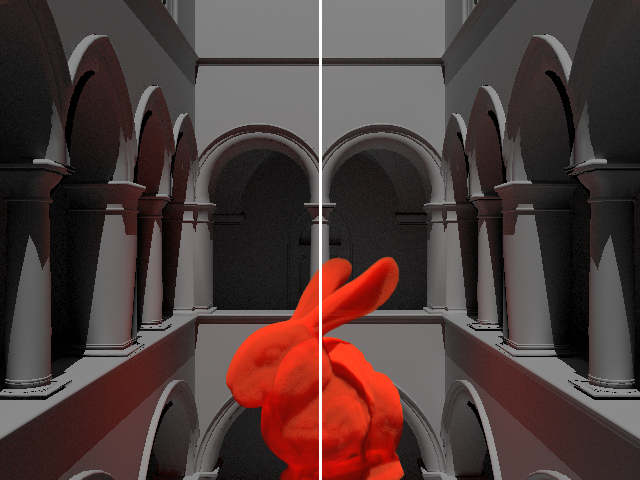
\includegraphics[width=100mm]{img/compare.png}
%    \caption{Bunny Scene comparison of the PCB extension (left) and traditional Monte Carlo results (right.)}
%    \label{fig:compare1}
%\end{figure}
%
%\begin{figure}[h!]
%    \centering
%    \includegraphics[width=100mm]{img/compare_head.png}
%    \caption{CT Head scene comparison of the PCB extension (left) and traditional Monte Carlo results (right.)}
%    \label{fig:compare2}
%\end{figure}
%
%Figures \ref{fig:compare1} and \ref{fig:compare2} show a comparison between Monte Carlo and PCBEX render results.  In order to objectively compare the image results, we used a perceptual image difference program called pdiff and ran the pair of images through in order to identify how close the two images were to each other.  The results are shown in tables \ref{tb:comparison_bunny} and \ref{tb:comparison_head}, which ranged from 2.1\% and 4.3\%.
%
%
%\begin{figure}[h!]
%    \centering
%    \includegraphics[width=80mm]{img/compare1_corrected.png}
%    \captionfonts
%    \caption{Zoomed image showing PCB extension (left) and Monte Carlo (right.)}
%    \label{fig:compare_close}
%\end{figure}
%
%\begin{figure}[h!]
%    \centering
%    \includegraphics[width=80mm]{img/compare_trad_corrected.png}
%    \captionfonts
%    \caption{Zoomed image showing traditional PCB (left) and PCB with extension (right.)  Note the visible color bleeding with our method.}
%    \label{fig:compare_trad}
%\end{figure}
%
%Figure~\ref{fig:compare_trad} compares the non-PCB Monte Carlo image with that of the traditional PCB renders, showing the clear lack of proper in-/out-scattering.  With the extended algorithm, however, the scenes look nearly identical.
%
%We noticed a dramatic jump in image difference between the $128^3$ resolution bunny model and the $512^3$ resolution model.  We believe that, because we used the same surfel sizes for all volume resolutions, that this discrepancy was caused by the complexity of the bunny volume.  Because the voxels were smaller, there is more room for error using larger lvoxels.  In real-world application we assume that lvoxels of much smaller size would be sampled and used in renders to mitigate this problem.
%
%We would like to note that there are a number of small artifacts in the PCB renders due to imprecision and incorrect surfel collisions.  It is important to note that, as past papers will attest, such issues are easily overcome and our artifacts are more due to implementation and time constraints than limits on the algorithm itself.
%
%\subsection{Scalability}
%
%The usefulness of the point cloud representation depends heavily on the cost of sampling the octree versus sampling the original scene geometry.  In our paper we assume that the cost of traversing the octree in a front-to-back order and sampling the point cloud is more efficient than sampling the polygonal meshes and integrating through the volumes.  Simpler scenes (such as the Cornell box) would only benefit from this algorithm given a complex or large volume to sample inside.
%
%Though we can compare and contrast specific sections of our algorithm to that of traditional Monte Carlo, the overall worst case run time is hard to evaluate.  Consider, first, the difficulty in evaluating overall scene complexity, which depends heavily on the acceleration structure being used (and all of the complexity that entails.)  We know for certain that the initial child lookup within our octree will give us a complexity of $n log(n)$.  Subsequent traversal of leaf nodes would be significantly less due to the recursive nature of our algorithm.
%
%We can estimate the total cost by multiplying the tests required for each leaf node by the total leaf nodes the ray will hit within an octree.  With that in mind, a theoretical worst case scene would involve a lot of close geometry (resulting in a deeply subdivided octree) and a camera orientation that would guarantee that most of the rays pass through most octree nodes.
%
%Using the point cloud to sample radiance in our test scenes showed a clear improvement over Monte Carlo sampling the original geometry.  With other companies like DreamWorks Animation and Disney employing the point-based color bleeding algorithm, it is clear they have found the point cloud representations to have faster evaluation times than the full scene geometry in production.  With the assumption that the point cloud does not get \textit{more} complex than the scene it is sampling, we can safely guess that we will see similar speedups.
%
%
%\section{Known Limitations}
%\label{sec:knownlimits}
%
%One problem we identified is that the algorithm assumes that there are no transparent polygonal surfaces in the scene.  Only completely opaque surfels are considered in our algorithm, and transparent polygonal surfaces would still return, not going further into the point cloud.  In fact, our surfel representation does not even have any notion of transparency.
%
%\vspace{5mm}
%
%We did not compare other volume integration/in-scattering acceleration structures which may have been a better suited comparison than that of strict integration of the participating media.  Other BSSRDF algorithms will follow a method similar to ours, creating nodes within the volume (or polygonal mesh) which approximate irradiance at each point.  These nodes allow for faster lookup of scatter lighting contribution within the object, allowing their algorithm to essentially skip proper volume integration (which is one of the most costly parts of the full Monte Carlo rendering algorithm.)
%
%\vspace{5mm}
%
%Because our volume phase function was isotropic (evaluating equal scatter in all directions,) we only had to keep track of one irradiance value in each lvoxel.  In a more complex system, we would use a better representation of the radiance scattering (perhaps through a spherical harmonic representation) which would push up the size of each lvoxel considerably.  This may cause the lvoxel point cloud to become more memory-intensive, but we do not foresee this as being excessively expensive.
%
%\section{Conclusion}
%In this paper, we discussed the necessity for proper global illumination approximations in renders, listed a number of algorithms that have attempted to do this but have fallen short specifically in volume scatter contributions, and presented an extension to the PCB algorithm by \cite{christensen:2008} which handles both scatter-in and scatter-out contributions.  The addition of the lvoxel paradigm to the already successful point-based color bleeding algorithm is shown to be a cost effective method of approximating and evaluating complex scatter functions based on participating media.  We obtained render speeds up to 36 times faster than that of pure Monte Carlo renders with a memory overhead between 2 to 5 MB with an image difference of less than 5\% across all tests.
%
%Computer graphics, be it photo-realistic or artistically leaning, relies heavily on the paradigms established in the physics of light in the real world.  Global illumination is just one of many areas of focus trying to better represent that light and its complex interactions in the abstract worlds we choose to bring to screen.  One can only imagine the leaps and bounds that computer graphics is destined to experience in the following years, but inevitably the obstacles boil down to the same subset of problems.  How to manipulate light and, by extension, color in order to make the viewer experience a story or emotion.
%
%%==============================================================================%
%\chapter{Future Work}
%
%
%As mentioned in Christensen's point based color bleeding article, surfels can be modified to ``gather'' light recursively from their position in the point cloud, allowing for simulated multi-bounce lighting.  This would require only a small change to the current algorithm, and would apply to volumes as well to allow very realistic scatter approximations in participating media.
%
%\vspace{5mm}
%
%In our tests, all participating media scatters light equally in all directions.  This is rarely the case, as volumes tend to have unique scatter functions.  We can simulate more complex surface scattering functions by creating spherical harmonic representations of the radiance at any specific point in the volume.  Our current implementation supports such an approach, but remains untested.
%
%\vspace{5mm}
%
%Typical implementations of the PCB algorithm include rougher estimations (usually in the form of a series of spherical harmonic coefficients) at higher levels in the octree, to be evaluated depending on that node's solid angle to our sample point.  Due to time constraints, we did not implement full multi-resolution representations of each node.  Including LVoxel data in that representation would be a trivial process.
%
%\vspace{5mm}
%
%As mentioned in Section \ref{sec:knownlimits}, we do not handle transparent objects in our algorithm.  This would likely involve a minor change to volume integration to include transparent surfels as well.
%
%\vspace{5mm}
%
%Our ray tracer runs a number of threads to split the image into multiple parts  in order to achieve simple parallelism.  Before the threads are created, however, we generate surfels and lvoxels sequentially.  Due to the nature of our octree implementation, we cannot add elements and still be thread safe, but this would not be a large obstacle.  Scenes like the sponza atrium would run a number of times faster if we were to parallelize our implementation more effectively.
%
%\vspace{5mm}
%
%Although for our purposes ray casting the scene to sample for surfels worked well, it is most certainly not an optimal algorithm.  Sampling the scene in a more geometry- aware fashion would lead to fewer samples and better results.  Subdividing the scene into smaller polygons and sampling the scene (say, one or two surfels per micro-polygon) would increase our coverage while decreasing unnecessary overlap.  We found that the simpler approach worked best for us, given our time frame, however it can most certainly be improved.
%
%\vspace{5mm}
%
%Because the color-bleeding effect in PCB focuses primarily on the point-cloud data, we are offered a unique opportunity to consider offloading the entire octree structure out-of-core in order to outsource the (still computationally complex) algorithm onto other machines, if not to on-board GPUs.  Taking advantage of a graphics processor's fast math and hardware rasterization would allow for much faster indirect-lighting evaluations.
%
%% ------------- End main chapters ----------------------
%
%\clearpage
%\bibliography{thesis}
%\bibliographystyle{plain}
%%\addcontentsline{toc}{chapter}{Bibliography}
%
%
%
%%==============================================================================%
%
%\section*{Image Results}
%
%\begin{figure}[h!]
%    \centering
%    \includegraphics[height=90mm]{img/sponza.png}
%    \captionfonts
%    \caption{The Sponza Atrium with the Stanford volumetric bunny.  In and Out-scattering are evident on the volume and on the surrounding atrium walls.}
%\end{figure}
%
%\begin{figure}[h!]
%    \centering
%    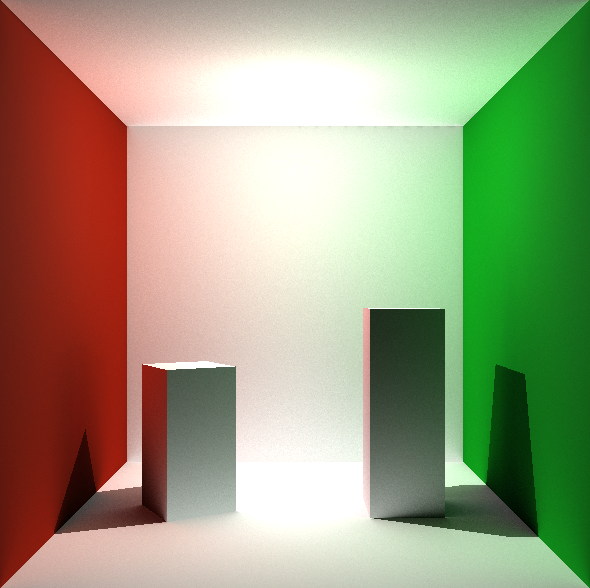
\includegraphics[height=90mm]{img/indirect_box_high.png}
%    \captionfonts
%    \caption{Example of point-based color bleeding without the volume extension algorithm.}
%\end{figure}
%
%\begin{figure}[h!]
%    \centering
%    \includegraphics[height=90mm]{img/two_sphere_indir.png}
%    \captionfonts
%    \caption{Example of a scene almost entirely in shadow, showing indirect lighting in play.}
%\end{figure}
%
%\begin{figure}[h!]
%    \centering
%    \includegraphics[height=90mm]{img/ketchup_good_corrected.png}
%    \captionfonts
%    \caption{Image exemplifying clear out-scattering from Stanford bunny volume.}
%\end{figure}
%
%\begin{figure}[h!]
%    \centering
%    \includegraphics[height=90mm]{img/bunny_spot/spot_right_new.png}
%    \captionfonts
%    \caption{Image exemplifying clear color bleeding next to the red wall in the bunny's shadow and correct transmittance through the bunny's hollow form.}
%\end{figure}
%
%\begin{figure}[h!]
%    \centering
%    \includegraphics[height=90mm]{img/one_side_corrected.png}
%    \captionfonts
%    \caption{The black occluding geometry in the center stops all but the light to the left to enter below.}
%\end{figure}
%
%\begin{figure}[h!]
%    \centering
%    \includegraphics[height=90mm]{img/bunny_glow.png}
%    \captionfonts
%    \caption{Illustrates how a light may act when placed within a hollow volumetric object.  The bunny is shown as slightly brighter, scattering light about the scene.}
%\end{figure}
%
%\begin{figure}[h!]
%    \centering
%    \includegraphics[height=90mm]{img/face1.png}
%    \captionfonts
%    \caption{Shows how CT scan data can be used to visualize scanned objects like a human face.  Subsurface scattering and transmittance through thin materials are evident.}
%\end{figure}



\end{document} %much faster 
